\section{ニューラルネットワーク}
\subsection{脳神経回路}
   人間の脳は神経細胞(neuron)とグリア細胞とから成り,情報処理の機能は主に神経細胞が行っているとされる。
  神経細胞は細胞体(soma)と軸索(axon)からなり,神経系を構成する。神経細胞同士のつながりを神経終端(もしくはシナプス)といい
  軸索末端が他の神経細胞の細胞体につながっている形になっている。細胞体と軸索末端との接合部について,
  細胞体側を樹状突起という。軸索末端と樹状突起は厳密に接合しているわけではなく,シナプス間隙と呼ばれる幅$20\sim 50\mathrm{nm}$の空間が
  存在している。また接合部において,軸索側の細胞膜をシナプス前膜(presynaptic cell),樹状突起側の細胞膜をシナプス後膜
  (postsynaptic cell)という。

   神経系を構成する細胞は以上のようになっているが,神経系の動作そのものは電気的な信号である。
  生体において電気現象は,細胞を構成する水溶液中のイオンによって行われる。細胞膜にはイオンポンプという
  イオンを選択的に輸送する機構があり,イオンポンプが能動的にイオンを輸送することで,膜を介した細胞同士で
  イオンが不均等な分布になるように維持される。イオンの不均等な分布は細胞膜を介した電位差を生じさせる。これを
  膜電位(membrane potential)という。膜電位は通常$-60\sim-80\mathrm{mV}$付近であり,この付近の電位を静止電位という。
  細胞は刺激に応じて膜電位を変化させ,この時の一過性の電位を活動電位という。活動電位が軸索末端に達することで
  シナプス前膜からイオンが流入し神経伝達物質という神経細胞における信号伝達を担う物質がシナプス間隙に放出される。
  放出された神経伝達物質をシナプス後膜側の受容体が受け入れることで異なる神経細胞に信号が伝わっていくのである。

   神経伝達物質の放出,吸収によって神経細胞の膜電位は変化する。神経伝達物質の蓄積によって膜電位は徐々に上昇し
  ある閾値に到達すると急激に変化し,その後静止電位に戻り,神経細胞の活性化という。これは神経伝達物質の放出に対応する。

   以上のことをまとめると,まず思考や感情を司る脳は神経細胞による神経系である。神経系の動作は電気信号であり,
  神経伝達物質の輸送によって神経細胞から他の神経細胞に伝わっている。そしてこの輸送は電気信号の過渡的な変化
  によって観測されるということである。
\bunseki{※米村祥裕}

\subsection{単純パーセプトロン}
  神経回路を模倣した演算モデルとして単純パーセプトロンというものが提案された。
  パーセプトロンは入力$\bm{x}=(x_i) \in \mathbb{R}^n $に対して$y=\{0,1\}$を出力する。
  パーセプトロンには入出力値以外に重み(weight)パラメータ$\bm{w}=(w_i) \in \mathbb{R}^n$
  ,閾値$\theta \in \mathbb{R}$がある。入力と出力との関係は式\ref{perceptron}で表される。
  
  \begin{equation}
    \label{perceptron}
    y =
    \left\{
    \begin{aligned}
      0 \quad &\sum_i{w_i x_i} < \theta \\
      1 \quad &\sum_i{w_i x_i} \geq \theta
    \end{aligned}
    \right.
  \end{equation}

  式\ref{perceptron}からわかるように,重みパラメータは入力の伝わりやすさを表している。
  入力値と重みパラメータとの積が閾値以上であれば1,閾値未満であれば0が出力される。
  式\ref{perceptron}は次の式\ref{perceptron2}のように書き直すことができ,この時のパラメータ$b\in \mathbb{R}$をバイアスという。

  \begin{equation}
    \label{perceptron2}
    y =
    \left\{
    \begin{aligned}
      0 \quad &\sum_i{w_i x_i} + b < 0 \\
      1 \quad &\sum_i{w_i x_i} + b \geq 0
    \end{aligned}
    \right.
  \end{equation}

  パーセプトロンによって実際に計算を構築するために,例として2入力AND回路について考えてみる。
  2入力AND回路の真理値表は表1のようになっている。

  \begin{table}[htb]
    \centering
    \caption{AND回路の真理値表}
    \begin{tabular}{|c|c|c|} \hline
      $x_1$ & $x_2$ & $y$ \\ \hline
      0 & 0 & 0 \\ \hline
      0 & 1 & 0 \\ \hline
      1 & 0 & 0 \\ \hline
      1 & 1 & 1 \\ \hline
    \end{tabular}
  \end{table}

  パーセプトロンで2入力AND回路を実現するには,パラメータを式\ref{andperceptronparameter}のように設定すればよい。

  \begin{equation}
    \label{andperceptronparameter}
    \left\{
      \begin{aligned}
        w_1 = 0.7 \\
        w_2 = 0.7 \\
        b = -1.0
      \end{aligned}
    \right.
  \end{equation}

  実際にすべての入力パターンについて重みパラメータと入力値との積の合計を計算してみる。

  \begin{table}[htb]
    \centering
    \caption{パーセプトロンによるAND回路の表現}
    \begin{tabular}{|c|c|c|c|} \hline
      $x_1$ & $x_2$ & $\sum_i{w_i x_i}+b$ & y \\ \hline
      0 & 0 & $-1$ & 0 \\ \hline
      0 & 1 & $-0.3$ & 0 \\ \hline
      1 & 0 & $-0.3$ & 0 \\ \hline
      1 & 1 & 0.4 & 1 \\ \hline
    \end{tabular}
  \end{table}

  同様に2入力OR回路もパラメータ$w_1 = 0.7, w_2 = 0.7, \theta = 0.5$などと設定すれば実現することができる。

  \bunseki{※米村祥裕}
\subsection{多層パーセプトロン}
  単純パーセプトロンでは2入力XOR(排他的論理和)回路は表現することができない。
  そこでパーセプトロンの出力を,他のパーセプトロンの入力とすることを考える。
  XOR回路はAND回路とNOT回路を組み合わせて作ることができるため,パーセプトロンを複数層に
  すれば実現することができる.
  
  \bunseki{※米村祥裕}
\subsection{順伝搬型ニューラルネットワーク}
パーセプトロンでは入力と重みパラメータとの積の総和が閾値以上であれば出力が1,閾値未満であれば0が出力される。
ニューラルネットワークを構成する計算要素(ユニットという)はより一般的に入出力を表現し,式\ref{NN}で表すことができる。

  \begin{equation}
    \label{NN}
    \begin{aligned}
    u ={}^t \bm{wx} + b \\
    y = f(u)
    \end{aligned}
  \end{equation}

  \begin{figure}[htb]
    \begin{center}
      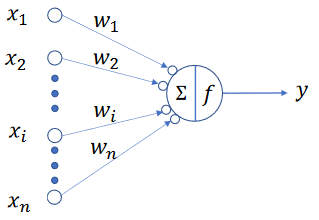
\includegraphics[clip, width=7.0cm]{./figure/neuralnetworkunit.png}
      \caption{ニューラルネットワークのユニット}
    \end{center}
  \end{figure}
  
  式\ref{NN}において$\bm{x} \in \mathbb{R}^n$は入力,$\bm{w} \in \mathbb{R}^n$は重みパラメータである。
  関数$f$を活性化関数という。パーセプトロンはニューラルネットワークの活性化関数にステップ関数を
  用いた特殊な場合であると考えることができる。

  パーセプトロンの場合と同様にニューラルネットワークも複数の層を形成させることができる。
  入力データを受け取る層を入力層,出力データを出力する層を出力層,入力層と出力層との間に存在する
  中間層という。

  \bunseki{※米村祥裕}
\subsection{活性化関数}
活性化関数は用途に応じて使い分けられる。ここでは代表的なものを挙げる。
  \bunseki{※米村祥裕}
\subsubsection{ステップ関数}
ステップ関数は$x\in \mathbb{R}$を入力として$y \in \mathbb{R}$を出力する。関数は式\ref{step_function}
で表される。入力層,中間層で主に使われる。パーセプトロンはステップ関数を利用していると考えることができる。
ステップ関数は連続でない関数であり,出力は0もしくは1である。そのため,後で後述するが,性能向上を考えたときに
関数の表現力に限界があるため,あまり使われなくなっている。

\begin{equation}
  \label{step_function}
  y = \left\{
    \begin{aligned}
      0 \quad x \leq 0 \\
      1 \quad x > 0
    \end{aligned}
  \right.
\end{equation}

\begin{figure}[htb]
  \begin{minipage}{0.5\hsize}
  \begin{center}
    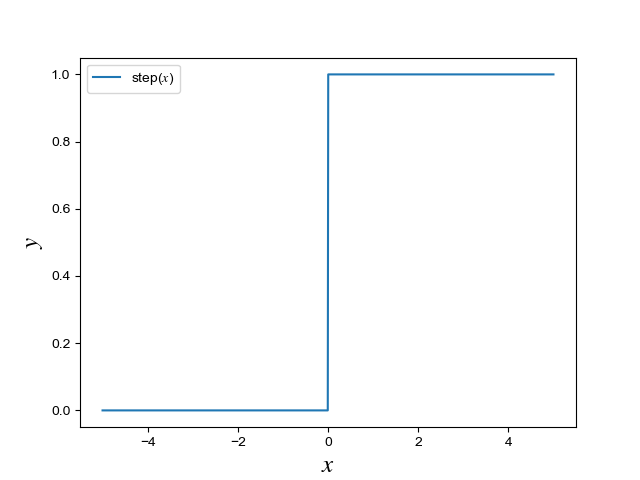
\includegraphics[clip, width=88mm]{./figure/step.png}
    \caption{ステップ関数の概形}
  \end{center}
  \end{minipage}
  \begin{minipage}{0.5\hsize}
  \begin{center}
    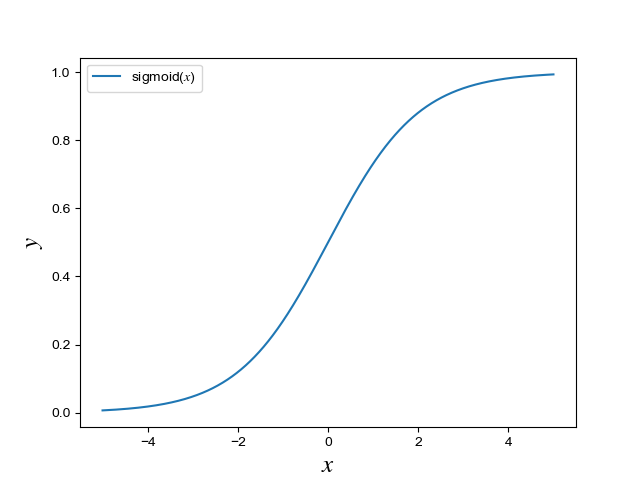
\includegraphics[clip, width=88mm]{./figure/sigmoid.png}
    \caption{シグモイド関数の概形}
  \end{center}
  \end{minipage}
\end{figure}

  \bunseki{※米村祥裕}
\subsubsection{シグモイド関数}
シグモイド関数は$x\in \mathbb{R}$を入力として$y \in \mathbb{R}$を出力する。関数は式\ref{sigmoid_function}で表される。
シグモイド関数はステップ関数とグラフの概形が似ているが,違いとしては連続かつ非線形であるという特徴がある。
また,シグモイド関数の勾配はすべての定義域で0にならない。この性質がニューラルネットワークの性能を向上させるうえで
重要となる。

\begin{equation}
  \label{sigmoid_function}
  y = \frac{1}{1+e^{-x}}
\end{equation}

  \bunseki{※米村祥裕}
\subsubsection{正則化線形関数(ReLU関数)}
正則化線形関数(ReLU)関数は$x\in \mathbb{R}$を入力として$y \in \mathbb{R}$を出力する。関数は式\ref{ReLU_function}で表される。
\begin{equation}
  \label{ReLU_function}
  y = \left\{
    \begin{aligned}
      0 \quad x < 0 \\
      x \quad x \geq 0
    \end{aligned}
  \right.
\end{equation}

  \bunseki{※米村祥裕}
\subsubsection{恒等関数}
恒等関数は出力層で主に用いられる関数である。入力$x\in \mathbb{R}$をそのまま出力として返す。

  \bunseki{※米村祥裕}
\subsubsection{ソフトマックス関数}
ソフトマックス関数は出力層で主に用いられる関数である。特に多クラス分類問題に用いられる。
ソフトマックス関数は$x\in \mathbb{R}^n$を入力として$y \in \mathbb{R}^n$を出力する。入力と出力との関係は次の式\ref{softmax_function}で表される。

\begin{equation}
\label{softmax_function}
y_k = \frac{e^{x_k}}{\sum_i^n e^{x_i}}
\end{equation}

$e^{x_k}$が大きいほど$y$は大きくなる。また$y_k$の総和は1になる。以上の性質を用いて,出力を
対応するクラスである確率であると解釈できる。そのため,$\b{max} \ e^{x_k}$に対応するクラスを出力とすることで,
入力に対していくつかのクラスを分類する問題に適用できる。

\bunseki{※米村祥裕}